\documentclass[12pt,letterpaper,addpoints]{exam}
\usepackage[utf8]{inputenc}
\usepackage{amsmath}
\usepackage{amsfonts}
\usepackage{amssymb}
\usepackage{amsthm}
\usepackage{graphicx}
\usepackage{tabularx}
\usepackage[left=2cm,right=2cm,top=2cm,bottom=2cm]{geometry}
\usepackage{multicol}
\usepackage{multirow,array}
\usepackage{newtxtext,newtxmath}
\usepackage{lastpage}
\usepackage{enumitem}
\newcolumntype{Y}{>{\centering\arraybackslash}X}
\firstpageheader{}{}{
\includegraphics[scale=0.5]{BHCClogoBW.jpg}\hspace{-40pt}\vspace{-50pt}}
\firstpagefooter{}{}{Page \thepage ~of \pageref{LastPage}}
\runningheader{ \textsc{Math 181 First Exam Practice}}{}{ \textsc{Fall 2018}}%{
\includegraphics[scale=.5]{BHCClogoBW.jpg}\vspace{-10pt}}%\hspace{-60pt}\vspace{-10pt}}
\runningheadrule
\runningfooter{}{}{Page \thepage ~of \pageref{LastPage}}
\renewcommand{\thequestion}{{\bf Q\arabic{question}}}
%\renewcommand{\questionlabel}{{\thequestion .}}
%\pointformat{\fbox{\themarginpoints \,pt}}
%\pointsinrightmargin
%\setlength{\rightpointsmargin}{1.5cm}
%\pointsinmargin
%\setlength{\marginpointssep}{10pt}

\begin{document}

\newcommand{\AND}{~\textsc{and}~}
\newcommand{\OR}{~\textsc{or}~}

\begin{center}
\text{ }\\
\vspace{40pt}
\textsc{{\Huge Math 181 First Exam Practice}}\\\vspace{5pt}
\textsc{{\large Spring 2019}}\\
\vspace{60pt}
\makebox[\textwidth]{\large Name:\enspace\hrulefill}\\
\vspace{40pt}
\fbox{\fbox{\begin{minipage}{6in}
\vspace{0.2in}
\begin{itemize}
\item Write your {\bf full name} on the line above.
\item Show your work. Incorrect answers with work can receive partial credit.
\item Attempt every question; showing you understand the question earns some credit.
\item If you run out of room for an answer, continue on the back of the page. Before doing so, write ``see back'' with a circle around it.
\item You can use 1 page (front and back) of notes.
\item You can use (and probably need) a calculator.
\item You can use the Geogebra Scientific Calculator instead of a calculator. You need to put your phone on {\bf airplane mode} and then within the application, start {\bf exam mode}; you should see a green bar with a timer counting up.
\item If a question is confusing or ambiguous, please ask for clarification; however, you will not be told how to  answer the question.
\item {\bf Box your final answer}.
\item A formula sheet is attached to this test.
\vspace{0.2in}
\end{itemize}
\end{minipage}
\begin{minipage}{0.2in}\text{ }\end{minipage}}}
\vfill
Do not write in this grade table.\\
\gradetable[h][questions]\\
\vfill
\end{center}

%%%%%%%%%%%%%%%%%%%%%%%%%%%%%%%%%%%%%%%%%%%%%%%%%%%%%%%%%%%%%%%%%%%%%%%%%%%%%%%

\newpage

\rhead{\textsc{Definitions and Formulas}}
{\bf Sample statistics:}\vspace{-10pt}
\begin{multicols}{2}\noindent
$n=\text{sample size} $\\
$x_i=\text{the $i$th value in a sample} $\\
$\bar x = \text{sample mean}$\\
$s = \text{sample standard deviation}$\\\\
$\bar x = \cfrac{\sum_{i=1}^n x_i}{n}$

\columnbreak \noindent
$Q_1$ = first quartile\\
$m$ = median\\
$Q_3$ = third quartile\\
IQR = inter-quartile range = $Q3-Q1$\\\\
$s = \sqrt{\cfrac{\sum_{i=1}^n (x_i-\bar x)^2}{n-1}}$ 
\end{multicols}

{\bf Population parameters:}\\
$\mu = \text{population mean}$\\
$\sigma = \text{population standard deviation}$\\

{\bf Probability:}\\
$\Omega = \text{set of all possible equally likely outcomes}$\\
$A = \text{event A, a set of outcomes}$\\
$A^c = \text{The complement of }A$\\
$B = \text{event B, another set of outcomes}$\\
$|A| = \text{size of set, number of outcomes in } A$\\
$P(A) = \text{probability of }A$\\
$P(A \AND B) = \text{probability of both $A$ and $B$}$\\
$P(A \OR B) = \text{probability of either $A$ or $B$ (or both)}$\\
$P(A | B) = \text{probability of $A$ given $B$}$\\\\
$P(A) = \cfrac{|A|}{|\Omega|}$\\\\
$0 \le P(A) \le 1$\\
$P(A \AND B) = P(A) \cdot P(B|A)$\\
$P(A \OR B) = P(A) + P(B) - P(A\AND B)$\\
$P(A^c) = 1 - P(A)$
\\\\
$A$, $B$ are disjoint (mutually exclusive) ~~$\iff~~P(A\AND B) = 0$\\
$A$, $B$ are non-disjoint ~~$\iff~~P(A\AND B) > 0$\\
$A$, $B$ are exhaustive ~~$\iff~~P(A\OR B) = 1$\\
$A$, $B$ are complements ~~$\iff$~~ $A$, $B$ are disjoint and exhaustive ~~$\iff$~~ $B=A^c$\\
$A$, $B$ are independent ~~$\iff~~P(A\AND B) = P(A)\times P(B) ~~\iff~~ P(A|B)=P(A)$\\

{\bf Random variables and distributions:}\\
$X=$ random variable \\
$x_i=$ the $i$th possible value of $X$. (Notice different meaning here vs. sample statistics.)\\
$k=$ number of possible values of $X$.\\
$E(X)=\mu=$ expected value of $X$\\
$\sigma=$ standard deviation of $X$\\
$\mu = \sum_{i=1}^k  x_i \cdot P(X=x_i) $\\
$\sigma = \sqrt{\sum_{i=1}^k (x_i-\mu)^2 \cdot P(X=x_i)}$


\newpage
\lhead{\textsc{Math 181}}
\rhead{\textsc{First Exam Practice}}
\begin{questions}

\question[10] An urn contains marbles. Each marble has a color and a pattern. The frequencies are shown in the contingency table.
\begin{center}
\begin{tabularx}{0.6\textwidth}{|Y|Y Y Y|Y|}\hline
          & red & green & blue & total\\ \hline
dotted    & 89  & 31    & 22  & 142 \\
striped   & 22 & 41 & 97 & 160 \\
checkered & 16 & 36 & 42 & 92  \\ \hline
total & 127 & 106 & 161& 394 \\ \hline
\end{tabularx}
\end{center}
\begin{parts}
\part What is the probability that a random marble is green?
\vfill
\part What is the probability that a random marble is striped and green?
\vfill
\part What is the probability that a random marble is striped or green?
\vfill
\part What is the probability that a random marble is striped given it is green?
\vfill
\part What is the probability that a random marble is green given it is striped?
\vfill
\end{parts}

\newpage

\question[10] Amira ran a study to see whether a rooting hormone increased the survival rate of roma-tomato cuttings (some plants can propagate by slicing off a branch and planting it). After collecting 18 cuttings, she dipped 9 (randomly selected) cuttings in rooting hormone and the others in water. After 4 weeks, she noted how many from each group survived.
\begin{center}
\begin{tabular}{c|c c}
& survived & died \\ \hline
hormone & 6 & 3 \\
water & 5 & 4 \\
\end{tabular}
\end{center}
\begin{parts}
\part Is this study observational or experimental?
\vfill
\part What is the sample?
\vfill
\part What are the cases (individuals)?
\vfill
\part What are the variables?
\vfill
\part Could a causal relationship be established by the study design?
\vfill
\part Was blinding used in this study?
\vfill
\part Which treatment (hormone or water) had a higher proportion surviving after 4 weeks?
\vfill
\part Describe the null hypothesis in the context of this study.
\vfill
\part Describe the alternative hypothesis in the context of this study.
\vfill
\part Has Amira shown, beyond a reasonable doubt, that hormone is more effective than water? Why or why not?
\vfill
\end{parts}

\newpage

\question[10] In 1888, the Swiss government collected data on 47 French-speaking provinces. Two of the variables were the percent of men engaged in agriculture and the percent of draftees earning top marks on an examination.
\vspace{-45pt}
\begin{center}
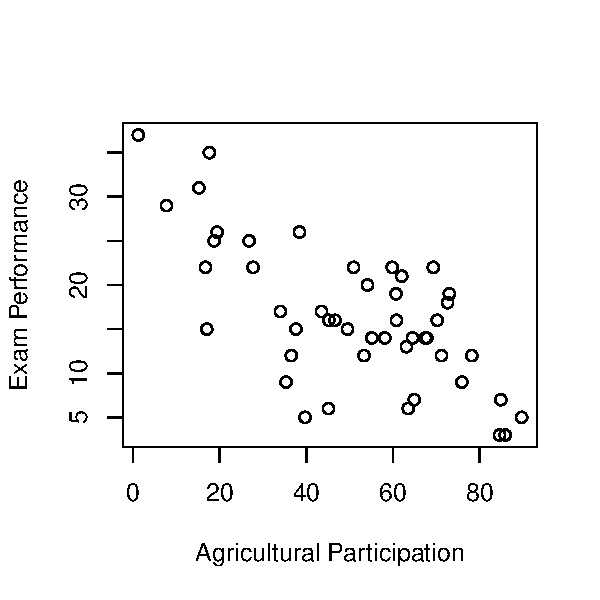
\includegraphics[scale=1]{figures/agex.pdf}
\end{center}
\begin{parts}
\part Which variable is the implied explanatory variable?
\vfill
\part Which variable is the implied response variable?
\vfill
\part What kind of association (positive, negative, or none) exists between these two variables?
\vfill
\part A friend suggests this study shows that agricultural participation causes lower exam performance. Is this a reasonable conclusion? Why or why not?
\vfill
\part What is a possible confounding variable?
\vfill
\end{parts}

\newpage

\question[10] A teacher has given an exam to 200 students, whose scores are shown in the histogram below. Please assume that the scores are almost all non-integer (this is meant to simplify the analysis by removing inclusive/exclusive concerns).
\vspace{-30pt}
\begin{center}
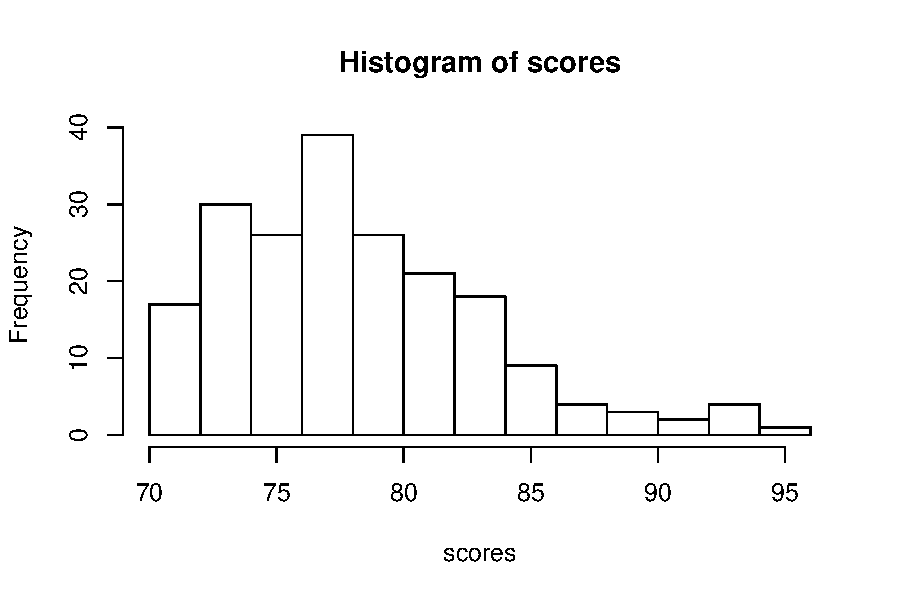
\includegraphics[scale=1]{figures/scores.pdf}
\end{center}
\begin{parts}
\part Estimate the proportion of students who scored between 70 and 74.
\vfill
\part Estimate the median.
\vfill
\part Is the mean higher or lower than the median? Why?
\vfill
\part Estimate the first quartile, $Q_1$.
\vfill
\part Estimate the third quartile, $Q_3$.
\vfill
\part Which of the following choices is the best estimate of the standard deviation.
\begin{checkboxes}
\choice 1
\choice 5
\choice 30
\choice 80
\choice 95
\end{checkboxes}
\end{parts}

\newpage

\question[10] Gary measured the masses (in grams) of 8 random oranges.
\begin{center}
\begin{tabular}{c c c c c c c c}
259 & 254 & 259 & 267 & 244 & 263 & 242 & 300
\end{tabular}
\end{center}
\begin{parts}
\part Find the sample mean ($\bar{x}$).
\vfill
\part Find the sample standard deviation ($s$).
\vfill
\vfill
\part Make a box plot. Label the features (with numbers).
\vfill
\vfill
\end{parts}

\newpage

\question[10] Jenn has a weighted die that rolls with probability distribution below. Let random variable $X$ represent the result of a roll.
\vspace{10pt}

{\large
\begin{tabular}{|c|c|}\hline 
$x_i$ & $P(X=x_i)$ \\ \hline
1 & 0.10\\
2 & 0.15\\
3 & 0.15\\
4 & 0.15\\
5 & 0.15\\
6 & 0.30\\\hline
\end{tabular}
}

\vspace{10pt}
\begin{parts}
\part What is $P(X = 6)$?
\vfill
\part Evaluate $P(2\le X \le 5)$.
\vfill
\part Evaluate the mean of the probability distribution. 
\vfill
\part Evaluate the standard deviation of the probability distribution. 
\vfill
\part Assume multiple rolls are independent, where $X_i$ is the result of the $i$th roll. Evaluate the probability $P(X_1 = 6 \AND X_2 = 6)$. In other words, what is the chance of rollings two 6s in a row?
\vfill
\part Evaluate $P(X_1 \ne 6 \AND X_2 \ne 6 \AND  X_3 \ne 6)$. In other words, what is the chance of rolling thrice and getting no 6s?
\vfill
\part Evaluate $P(X_1 = 6 \OR X_2 = 6 \OR X_3 = 6)$. In other words, what is the chance of rolling thrice and getting at least one 6? 
\vfill
\part If you want a series of rolls to average between 3 and 5, and you get to choose the number of rolls before starting, should you choose 10 rolls or 100 rolls? Why?
\vfill
\part If you want a series of rolls to average between 1 and 3, and you get to choose the number of rolls before starting, should you choose 10 rolls or 100 rolls? Why?
\vfill
\end{parts}

\newpage

\question[10] In a kennel, 80\% of dogs are good dogs; the others are bad dogs. If a dog is good, it has a 70\% chance of sitting on command. If a dog is bad, it has a 40\% chance of sitting on command. You meet a dog, and it {\bf does not} sit on command. What is the chance it is a good dog given it didn't sit on command?
\begin{parts}
\part Draw a tree diagram.
\vfill
\vfill
\part Make a contingency table.
\vfill
\part Determine the probability the dog is good given it {\bf did not} sit on command.
\vfill
\end{parts}

\newpage

\question[10] Let random variable $Y$ be continuously distributed by the probability density function shown below. Notice the entire area is split into 100 percentile squares.
\begin{center}
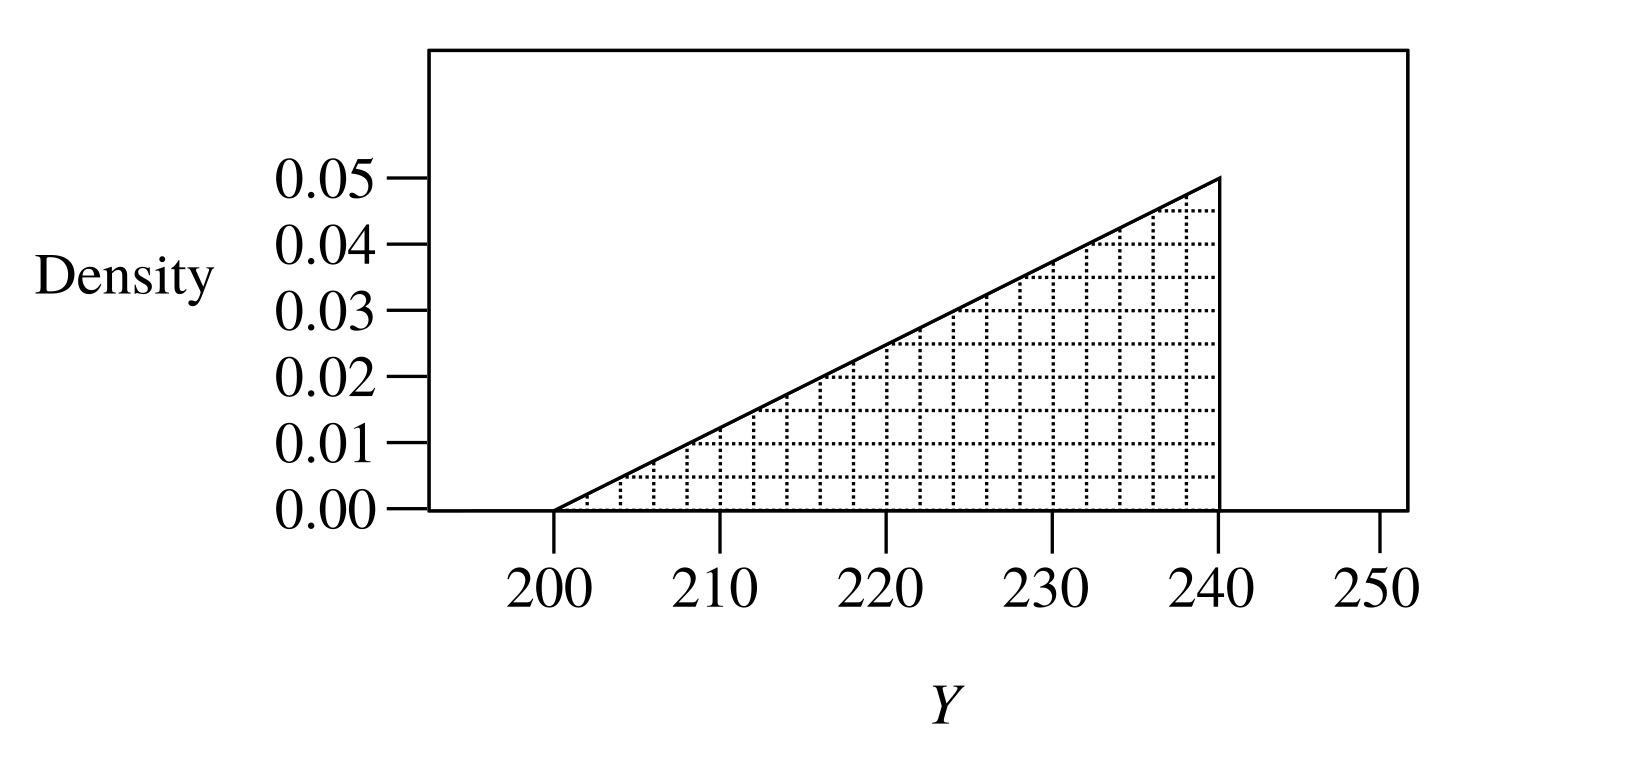
\includegraphics[scale=1]{figures/cd.png}
\end{center}
\begin{parts}
\part Evaluate $P(Y=212)$. In other words, what is the probability that $Y$ is exactly 212?
\vfill
\part Evaluate $P(Y<212)$. In other words, what is the probability that $Y$ is less than 212?
\vfill
\part Evaluate $P(220<Y<224)$. In other words, what is the probability that $Y$ is between 220 and 224?
\vfill
\part Estimate $Q_1$.
\vfill
\part Estimate the median.
\vfill
\part Is the mean lower than, equal to, or greater than the median?
\vfill
\end{parts}

\end{questions}
\end{document}